\documentclass[10pt,conference,compsocconf]{IEEEtran}

\usepackage{hyperref}
\usepackage{graphicx}	% For figure environment
\usepackage{xspace}
\usepackage{mathtools}
\usepackage{url}


\begin{document}
\title{LC3 Compressive Strength Analysis}
\author{
  David Alonso del Barrio, Francisco Javier Blázquez Martínez, Andrés Montero Ranc\\
  \textit{Construction Materials Laboratory, EPFL, Switzerland}
}

\maketitle

\begin{abstract}
LC3 stands for Limestone Calcined Clay Cement, it is the newest type of cement that offers an alternative for environmental sustainability, it is made with calcined clay, this material can be found in abundance, it is an ecological cement that contains less clinker and uses less fuel in its production, therefore reducing CO2 emissions by up to 30\%.
\end{abstract}

\section{Introduction}

The aim of this project has been to help the construction materials laboratory to build a machine learning model that will provide them with information on which characteristics of clay have the greatest impact on the compressive strength of cement, and also to be able to answer questions such as: "if I want a resistance of \% what quantities of each characteristic of clay do I need. 
\section{Data preprocessing }
At the beginning of the project we were given several sets of data, and our first task was to see, without any pre-processing of the data we had, what information we could work with. We quickly realised that we had little data available. We had about 50-60 types of clay and each had about 20 different characteristics. We also observed that, in many of the clays, the characteristics associated with them were MV, so we had little data and quite a lot of MV.
What attracted us to the project was that the tutor told us that most of these data had never been treated, so we could provide a lot of information to the laboratory, and help them in some way which was the main objective.
The difficulty in processing the data was in their structure. They provided us with a series of Excel files, which had been prepared by a person who was no longer in the laboratory, and they were not at all intuitive and rather messy, so our first task had to be to try to build much clearer datasets to be able to work with them.
The pre-processing of the data took a lot of time and effort as these datasets contained values from which we did not know their origin, and in many cases, the averages calculated in one excel did not coincide with the averages calculated in the other, so in collaboration with the project tutor we managed to structure the data in such a way that we could work with them.
 To summarise what the data sets consisted of, we differentiated between two parts: on the one hand, we had the compressive strength of the cement manufactured with the different types of clay, and on the other, the characteristics associated with each type of clay, i.e. our dependent variable was the compressive strength, and our independent variables were the characteristics of the clays. It is important to note that the difference between the two sets of data is that, in one of them, we had the average compressive strength and standard deviation of days 1, 3, 7, 28 and 90, for each of the clays used, and in the other, we had all the measurements with which the averages and standard deviation had been calculated. 
This allowed us to elaborate three lines of development of the work, on the one hand to study the problem from the averages and the standard deviation and on the other hand to work with all the measures that we had available.
\section{Models and Methods}
In the case of the work with both the averages and all the measures, we have carried out the same methods, but in the case of the standard deviations we have followed a different approach. We will now explain the methods used:
\subsection{Correlated features}
We studied the correlation between the different characteristics, and the relationship between the characteristics and the compressive strength, and as a data to highlight, we saw that the level of kaolinite had a strong correlation with the compressive strength.
\subsection{R2 and MSE}
Then, we designed a series of functions, to obtain the combination of variables that gave us a better R square, and a lower mean square error. For each day we obtained relationships of different variables, but in all of them we found the Kaolinite level, which was the characteristic with the greatest impact on the compressive strength. 
The aim of these functions was to know which characteristics we should work with when doing the linear regression. We considered that, as a first model, we should use linear regression with only one feature, in this case the Kaolinite level.
The R-square is a statistical measure of how close the data is to the adjusted regression line, and the closer to 1 the better the line fits the data.The adjusted R-squared is a modified version of R-squared that has been adjusted for the number of predictors in the model. The adjusted R-squared increases only if the new term improves the model more than would be expected by chance. It decreases when a predictor improves the model by less than expected by chance. Since in our case we only had a few points, we used an adjusted r-squared that provides us with a way to penalize equations that take into account many variables. In this way we avoid overfitting.
\subsection{Leave one out validation}
As it is true, as we increase the degree of complexity or add more variables to our regression, we are going to get a better R2, but we could be having overfitting. To avoid this, we thought about cross validation, but having so little data we had to opt for a particular type of cross validation: leave out cross validation. In this type of validation the number of folds is equal to the number of instances in the data set. Therefore, the learning algorithm is applied once for each instance, using all other instances as a training set and using the selected instance as a single element test set
\subsection{Linear Regression}
\subsubsection{Ordinary Least Squares}
We started with simple models, using ordinary least squares to obtain the relation between compressive strength and kaolinite level, which was the feature with the best performance.
\subsubsection{Weighted Least Squares}
\begin{figure*}[tbp]
  \centering
  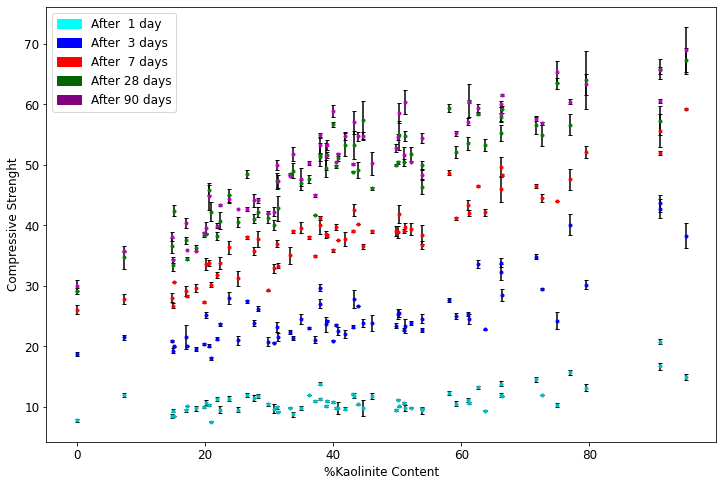
\includegraphics[width=\textwidth]{figures/cstrength-std.png}
  \caption{Compressive strength in relation of Kaolinite content for days 1, 3 , 7, 28, 90 (each data-point was provided as a mean of 3 to 7 other samples we had not access to and its error-bars correspond to the standard deviation obtained for those means). }
  \vspace{-3mm}
  \label{fig:cstrength-std}
\end{figure*}
Data provided us with a standard deviation for each mean (datapoint for compressive strength) [Figure~\ref{fig:denoise-wavelet}], so we decided to carry out another approach: modeling the data weighting these means with their standard deviation. We had to come up with a way to model our data in which the larger the standard deviation was, the less importance the sample had to have. 
To do this, we opted to use a tailor-made version of the method the WLS (Weighted Least Squares) provided by the \textit{statsmodels} library \cite{sm:wls}. \textit{The weighted least squares method is a generalization of the ordinary least squares and linear regression in which the errors covariance matrix is allowed to be different from an identity matrix [...]}

\textit{If the errors are uncorrelated and have equal variance, then the minimum of the function}
\newline
$
S({\boldsymbol{\beta }})=\sum_{i}{r_{i}({\boldsymbol{\beta }})^{2}}
$,
\textit{is found when}
$
\displaystyle{\frac{\partial S({\hat {\boldsymbol {\beta }}})}{\partial \beta _{j}}}=0
$
\textit{(defining ${\displaystyle {\boldsymbol {\hat {\beta }}}}$). }
\newline
\newline
\textit{[...] The Gauss–Markov theorem shows that, when this is so, Beta is a "best linear unbiased estimator" (BLUE). If, however, the measurements are uncorrelated but have different uncertainties, a modified approach might be adopted. Aitken showed that when a weighted sum of squared residuals is minimized, Beta is the BLUE if each weight is equal to the reciprocal of the variance of the measurement.}\cite{wiki:wls}

So the usual way to use this method is to provide the reciprocal of the variance of the measurement. That is, concerning the rest of the samples. As in our case, the data samples had their standard deviation,  one way to introduce this variance in our model would be to take the current value of the variance of each sample concerning its partners and multiply it by the standard deviation provided squared. And so, obtaining the weights that would give us the BLUE. 

To simplify, for this report we limit ourselves to a modified approach in which we normalize the standard deviations given and input the inverse value to our \textit{statsmodels} module.

\subsection{Non Linear Models}
Continuing with that approach, and adding a little more complexity, we have used feature augmentation, and we have done the regression with kaolinite, kaolinite square and another variable. We have chosen to make feature augmentation of the Kaolinite because it is the feature that has the greatest relationship to compressive strength, as we have seen in the correlation analysis as in the MSE and R2 analysis.  And then based on these analyses we have selected another feature that will allow us to improve the model.
\subsection{Confidence Intervals}
The objective of this method is to provide a more mathematical analysis of the confidence we can expect from our models, and give a better answer to the questions the lab wants our model to answer. This applies to the models used with and without the standard deviation given.
\section{Results}
\subsection{AVERAGE}
The main conclusions we drew from this first regression were that there were few more we could improve at the 7th day using only the kaolinite content, data distribution was quite a straight line.
For 1st and 3rd day the problem was more the sparsification of the points than the lack of expressivity of the model, and for 28th and 90th day until 40\% of kaolinite content the compression strength increases linearly and then stabilizes.

Having seen the results, we tried kaolinite squared, and we achieved better models for 28th and 90th day compressive strength obtained,and we saw a potential overfitting for 1st and 3rd day measurements because we were not increasing the compressive strength with the increase of Kaolinita for small contents.(ESTO QUITARLO, COMO SI NO HUBIERA PASADO NADA, O EXPLICAR COMO SE HA QUITADO EL OVERFITTING) 
Regarding the selection of a feature to complement Kaolinite, we see that "Dv50", and calcium oxide in the early days is a good choice, and "BET\_specific\_surface" and span for the later days. It is true that "D10" and "D90" are the characteristics with the highest R2 and lowest MSE, but we do not have enough data to consider them valid.
CREO QUE SERÍA CONVENIENTE EXPLICAR QUE ES "D-50,10", PARA FACILITAR LA LECTURA, PERO NO ME ACUERDO QUE ERAN.

\subsection{STANDARD DEVIATION}

The results obtained from the modelling with the standard deviation marked a notable difference with the model obtained only with the means. Theoretically, this model is closer to BLUE. 

\begin{figure}[htbp]
  \centering
  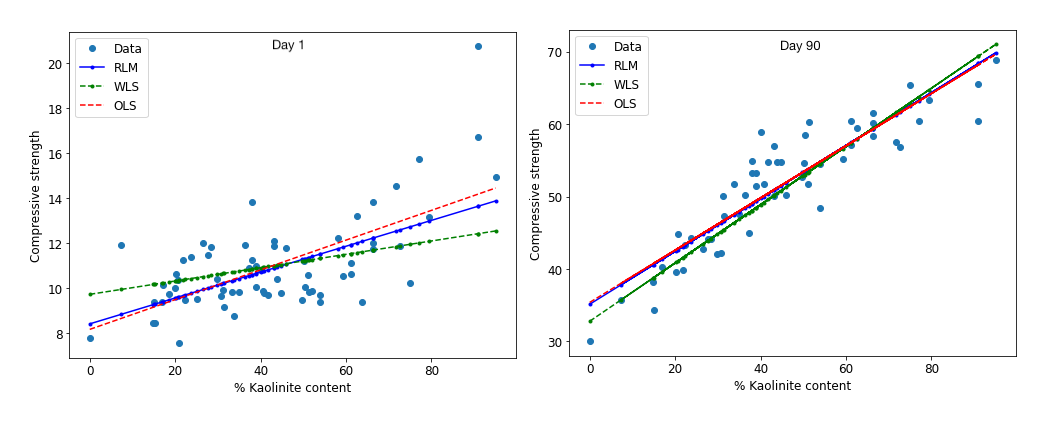
\includegraphics[width=\columnwidth]{figures/lr-ols-wls-rls-d1-d90.png}
  \vspace{-3mm}
  \caption{.}
  \label{fig:denoise-wavelet}
\end{figure}

\subsection{ALL MEASUREMENTS}
When analysing the regression using all available measures, we have observed similar behaviour to that observed with averages(greater randomness on days 1 and 3, linear response on day 7, and non-linear behavior on days 28 and 90) , but having more data we have been able to have greater certainty in representing the confidence intervals, and this was the main reason for using all the data.
regarding the selection of a feature to complement the Kaolinite, we can see that "D10", "D90", "span" and "BET\_specific\_surface" are characteristics with great predictive importance. However, as in the case of averages, we do not have enough data with measures "D10" and "D90" to trust them. So we choose "span" and "BET\_specific\_surface" to create models along with the kaolinite content.
\section{Discussion}
\begin{itemize}
\item The scarcity of data has made us opt for simple models, but which in turn can answer the questions posed to us from the laboratory.

\item Kaolinite content has a strong relationship to compressive strength.
\item On days 1 and 3 we see a little more random behaviour, but from day 7 we see a much more stable behaviour. This may be due to the setting time. This is why we consider that it makes more sense to work with the data from the first week, when studying the behavior of clays and making decisions about which clay to use.
\item On the 28th and 90th days, we clearly see how for low values of Kaolinite, there is a linear relationship with the compressive strength but for intermediate and high values of Kaolinite the compressive strength tends to stabilise at one value, so the non-linear model is best suited to the data.

\end{itemize}
\section{The Structure of a Paper}
\label{sec:structure-paper}

Scientific papers usually begin with the description of the problem,
justifying why the problem is interesting. Most importantly, it argues
that the problem is still unsolved, or that the current solutions are
unsatisfactory. This leads to the main gist of the paper, which is
``the idea''. The authors then show evidence, using derivations or
experiments, that the idea works. Since science does not occur in a
vacuum, a proper comparison to the current state of the art is often
part of the results. Following these ideas, papers usually have the
following structure:
\begin{description}
\item[Abstract] \ \\
  Short description of the whole paper, to help the
  reader decide whether to read it.
\item[Introduction] \ \\
  Describe your problem and state your
  contributions.
\item[Models and Methods] \ \\
  Describe your idea and how it was implemented to solve
  the problem. Survey the related work, giving credit where credit is
  due.
\item[Results] \ \\
  Show evidence to support your claims made in the
  introduction.
\item[Discussion] \ \\
  Discuss the strengths and weaknesses of your
  approach, based on the results. Point out the implications of your
  novel idea on the application concerned.
\item[Summary] \ \\
  Summarize your contributions in light of the new
  results.
\end{description}


\section{Tips for Good Writing}
\label{sec:tips-writing}

The ideas for good writing have come
from~\cite{editor10,jones08,anderson04}.

\subsection{Getting Help}
One should try to get a draft read by as many friendly people as
possible. And remember to treat your test readers with respect. If
they are unable to understand something in your paper, then it is
highly likely that your reviewers will not understand it
either. Therefore, do not be defensive about the criticisms you get,
but use it as an opportunity to improve the paper. Before your submit
your friends to the pain of reading your draft, please \emph{use a
  spell checker}.

\subsection{Abstract}
The abstract should really be written last, along with the title of
the paper. The four points that should be covered~\cite{jones08}:
\begin{enumerate}
\item State the problem.
\item Say why it is an interesting problem.
\item Say what your solution achieves.
\item Say what follows from your solution.
\end{enumerate}

\subsection{Figures and Tables}



Use examples and illustrations to clarify ideas and results. For
example, by comparing Figure~\ref{fig:denoise-fourier} and
Figure~\ref{fig:denoise-wavelet}, we can see the two different
situations where Fourier and wavelet basis perform well. 

\subsection{Models and Methods}
The models and methods
section should describe what was
done to answer the research question, describe how it was done,
justify the experimental design, and
explain how the results were analyzed.

The model refers to the underlying mathematical model or structure which 
you use to describe your problem, or that your solution is based on. 
The methods on the other hand, are the algorithms used to solve the problem. 
In some cases, the suggested method directly solves the problem, without having it 
stated in terms of an underlying model. Generally though it is a better practice to have 
the model figured out and stated clearly, rather than presenting a method without specifying 
the model. In this case, the method can be more easily evaluated in the task of fitting 
the given data to the underlying model.

The methods part of this section, is not a step-by-step, directive,
protocol as you might see in your lab manual, but detailed enough such
that an interested reader can reproduce your
work~\cite{anderson04,wavelab}.

The methods section of a research paper provides the information by
which a study's validity is judged.
Therefore, it requires a clear and precise description of how an
experiment was done, and the rationale
for why specific experimental procedures were chosen.
It is usually helpful to
structure the methods section by~\cite{kallet04methods}:
\begin{enumerate}
\item Layout the model you used to describe the problem or the solution.
\item Describing the algorithms used in the study, briefly including
  details such as hyperparameter values (e.g. thresholds), and
  preprocessing steps (e.g. normalizing the data to have mean value of
  zero).
\item Explaining how the materials were prepared, for example the
  images used and their resolution.
\item Describing the research protocol, for example which examples
  were used for estimating the parameters (training) and which were
  used for computing performance.
\item Explaining how measurements were made and what
  calculations were performed. Do not reproduce the full source code in
  the paper, but explain the key steps.
\end{enumerate}

\subsection{Results}

Organize the results section based on the sequence of table and
figures you include. Prepare the tables and figures as soon as all
the data are analyzed and arrange them in the sequence that best
presents your findings in a logical way. A good strategy is to note,
on a draft of each table or figure, the one or two key results you
want to address in the text portion of the results.
The information from the figures is
summarized in Table~\ref{tab:fourier-wavelet}.

\begin{table*}[htbp]
  \centering
  \begin{tabular}[c]{|l||l|l|l|}
    \hline
    Basis&Support&Suitable signals&Unsuitable signals\\
    \hline
    Fourier&global&sine like&localized\\
    wavelet&local&localized&sine like\\
    \hline
  \end{tabular}
  \caption{Characteristics of Fourier and wavelet basis.}
  \label{tab:fourier-wavelet}
\end{table*}

When reporting computational or measurement results, always
report the mean (average value) along with a measure of variability
(standard deviation(s) or standard error of the mean).


\section{Tips for Good Software}
\label{sec:tips-software}

There is a lot of literature (for example~\cite{hunt99pragmatic} and
\cite{spolsky04software}) on how to write software. It is not the
intention of this section to replace software engineering
courses. However, in the interests of reproducible
research~\cite{schwab00}, there are a few guidelines to make your
reader happy:
\begin{itemize}
\item Have a \texttt{README} file that (at least) describes what your
  software does, and which commands to run to obtain results. Also
  mention anything special that needs to be set up, such as
  toolboxes\footnote{For those who are
  particularly interested, other common structures can be found at
  \url{http://en.wikipedia.org/wiki/README} and
  \url{http://www.gnu.org/software/womb/gnits/}.}.
\item A list of authors and contributors can be included in a file
  called \texttt{AUTHORS}, acknowledging any help that you may have
  obtained. For small projects, this information is often also
  included in the \texttt{README}.
\item Use meaningful filenames, and not \texttt{temp1.py},
  \texttt{temp2.py}. 
\item Document your code. Each file should at least have a short
  description about its reason for existence. Non obvious steps in the
  code should be commented. Functions arguments and return values should be described.
\item Describe how the results presented in your paper can be reproduced.
\end{itemize}


\subsection{\LaTeX{} Primer}
\label{sec:latex-primer}

\LaTeX{} is one of the most commonly used document preparation systems
for scientific journals and conferences. It is based on the idea
that authors should be able to focus on the content of what they are
writing without being distracted by its visual presentation.
The source of this file can be used as a starting point for how to use
the different commands in \LaTeX{}. We are using an IEEE style for
this course.

\subsubsection{Installation}

There are various different packages available for processing \LaTeX{}
documents.
On OSX use Mac\TeX{}
(\url{http://www.tug.org/mactex/}). On Windows, use for example Mik\TeX{} (\url{http://miktex.org/}).

\subsubsection{Compiling \LaTeX{}}
Your directory should contain at least~4 files, in addition to image
files. Images should be in \texttt{.png}, \texttt{.jpg} or
\texttt{.pdf} format.
\begin{itemize}
\item IEEEtran.cls
\item IEEEtran.bst
\item groupXX-submission.tex
\item groupXX-literature.bib
\end{itemize}
Note that you should replace groupXX with your chosen group name.
Then, from the command line, type:
\begin{verbatim}
$ pdflatex groupXX-submission
$ bibtex groupXX-literature
$ pdflatex groupXX-submission
$ pdflatex groupXX-submission
\end{verbatim}
This should give you a PDF document \texttt{groupXX-submission.pdf}.

\subsubsection{Equations}

There are three types of equations available: inline equations, for
example $y=mx + c$, which appear in the text, unnumbered equations
$$y=mx + c,$$
which are presented on a line on its own, and numbered equations
\begin{equation}
  \label{eq:linear}
  y = mx + c
\end{equation}
which you can refer to at a later point (Equation~(\ref{eq:linear})).

\subsubsection{Tables and Figures}

Tables and figures are ``floating'' objects, which means that the text
can flow around it.
Note
that \texttt{figure*} and \texttt{table*} cause the corresponding
figure or table to span both columns.



\section{Summary}

The aim of a scientific paper is to convey the idea or discovery of
the researcher to the minds of the readers. The associated software
package provides the relevant details, which are often only briefly
explained in the paper, such that the research can be reproduced.
To write good papers, identify your key idea, make your contributions
explicit, and use examples and illustrations to describe the problems
and solutions.

\section*{Acknowledgements}
The author thanks Christian Sigg for his careful reading and helpful
suggestions.

\bibliographystyle{IEEEtran}
\bibliography{literature.bib}

\end{document}
